\section{Results}
\label{s:results}
In this section we present a preliminary evaluation of the proposed method dealing with the estimation of elastic parameters of a deformable 
object. The evaluation was performed using synthetic data which provide the ground truth that is used to assess the accuracy of the 
estimation. The section is structured as follows: first, we describe the testing scenarios used for the evaluation. Next, we 
present the quantified results demonstrating the accuracy of the estimations in terms of expected value and standard deviation. Finally, 
we focus on the performance of the actual implementation of the method. 

\subsection{Testing Scenarios}
\label{sr:scenarios}
The synthetic data used for the evaluation of the data assimilation technique allowing for the estimation of a large number of parameters
was generated using \emph{forward}, \ie\ a simulation executed for a given parametrization, based on the finite element corotational formulation of non-linear elasticity. 
Two tetrahedral meshes were generated for an object with cylindric shape using the Gmsh tool~\footnote{\url{http://geuz.org/gmsh/}}. 
The first mesh $\msa$ discretizing a cylinder ($l_1$=\SI{24}{\cm} and $r_1$=\SI{2}{\cm} being the length and radius) 
is divided into three segments and consists of 770 elements; the second mesh $\msb$ represents a domain of cylinder 
with $l_2$=\SI{30}{\cm} and $r_2$=\SI{2}{\cm}, divided into 10 segments composed of 4245 elements in total. 

Both meshes are first employed in the forward simulation using SOFA as follows: each cylinder is fixed on the lateral facets
using homogeneous Dirichlet conditions and the gravity is applied to the object having density $\rho$ = \SI{1000}{\kg\per\cubic\metre}.
The behavior of each cylinder is modeled with corotation finite element formulation. While constant Poisson's ratio ($\nu$ = \SI{0.45})
is applied over the entire volume of both cylinders, different Young's modulus is attributed to each segment mimicking the 
heterogeneous nature of tissues. 
The simulation is performed using quasi-static solver where in each step, the gravity is increased by 1/100 of the target value, 
thus requiring 100 steps to reach the final deformation. Single linearization per simulation step is performed and the 
linearized system of equations is factorized using LDL solver Pardiso~\footnote{http://www.pardiso-project.org/}. 
In each step, the actual position of all nodes is stored in a file which later serves as the source of observations. The deformed configurations are depicted in Fig.~\ref{f:cylScreens}. 

\begin{figure*}[th]%
\centering%
\subfigure[]{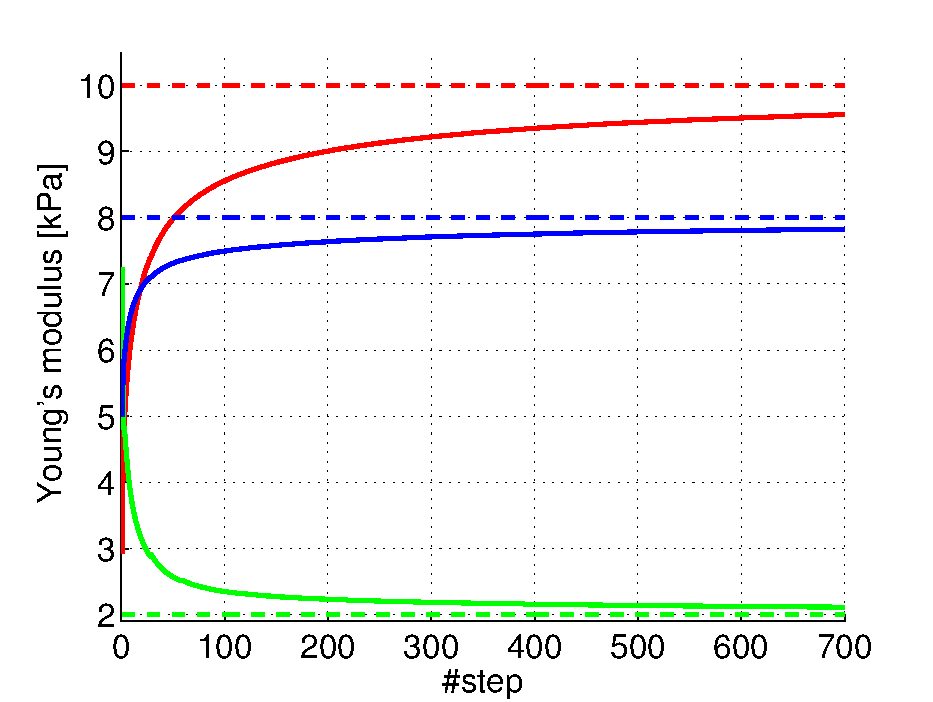
\includegraphics[width=.32\textwidth]{figs/cyl3_par.pdf}}
\hfill
\subfigure[]{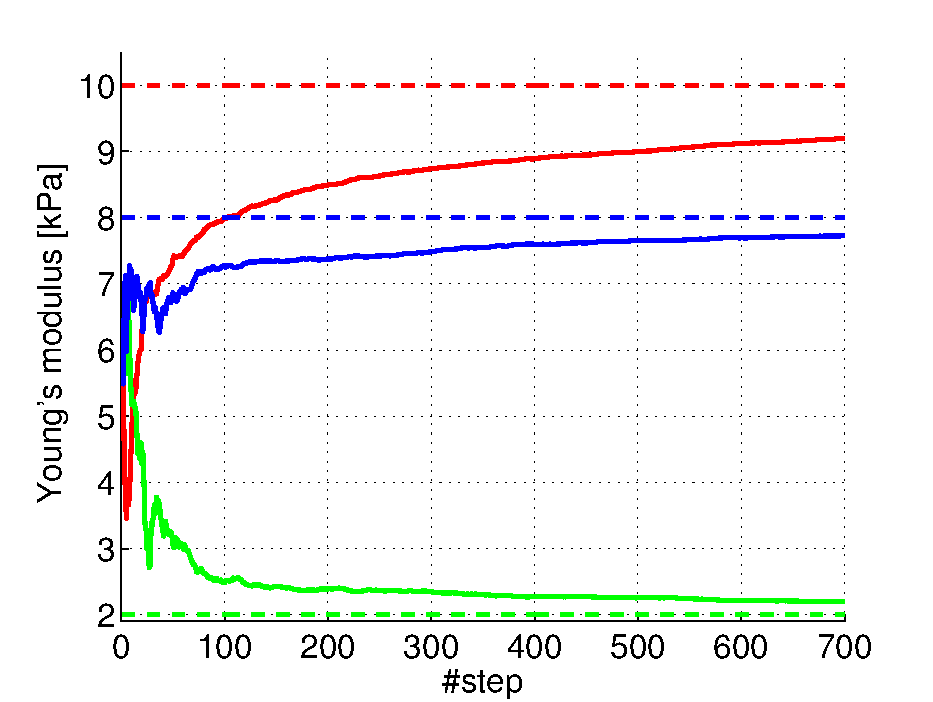
\includegraphics[width=.32\textwidth]{figs/cyl3ns_par.pdf}}
\hfill
\subfigure[]{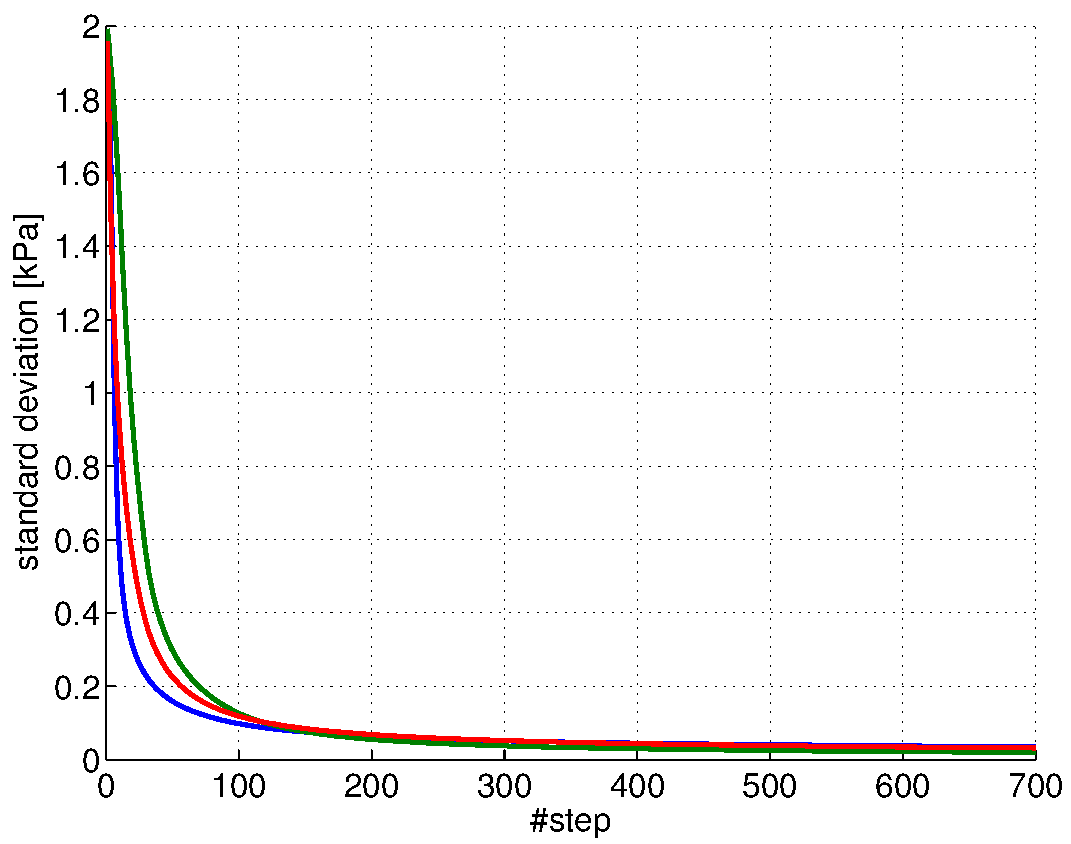
\includegraphics[width=.32\textwidth]{figs/cyl3ns_var.pdf}}
\caption{Results of the estimation of parameters for $\msa$: Three parameters are estimated, each associated to 
one segment. Figures (a) and (b) show the evolution of the parameter estimation as the function of the quasi-static 
incremental gravity loading without and with noise added to the observations, respectively. The dashed lines indicate the ground-truth 
and the estimation starts in the undeformed configuration. The plot (c) shows the evolution of standard deviation 
associated to each parameter and their combinations, respectively.}
\label{f:cyl3Estim}
\end{figure*}

\begin{figure*}[t!]%
\centering%
\subfigure[]{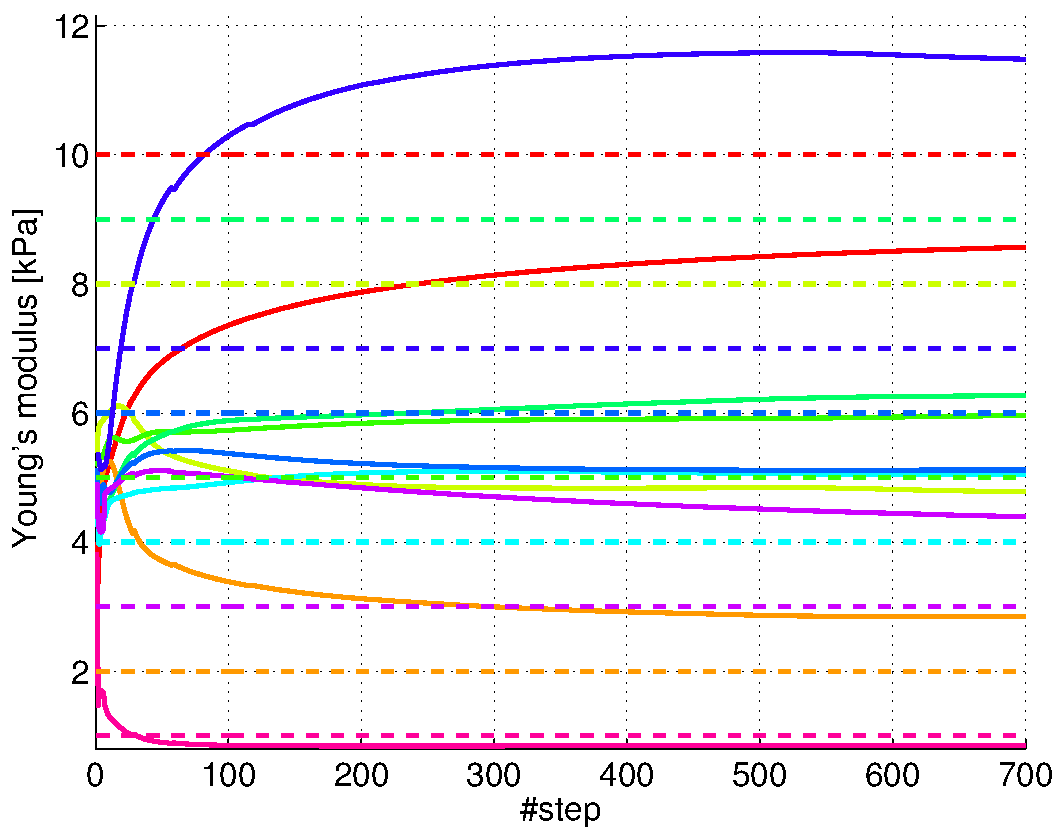
\includegraphics[width=.32\textwidth]{figs/cyl10_par.pdf}}
\hfill
\subfigure[]{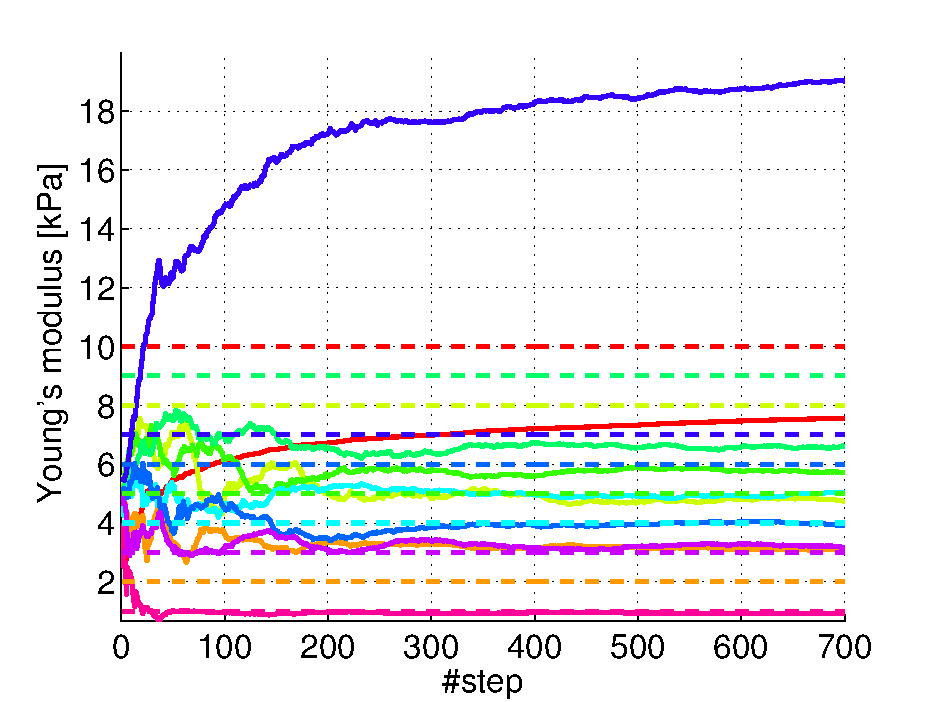
\includegraphics[width=.32\textwidth]{figs/cyl10ns_par.pdf}}
\hfill
\subfigure[]{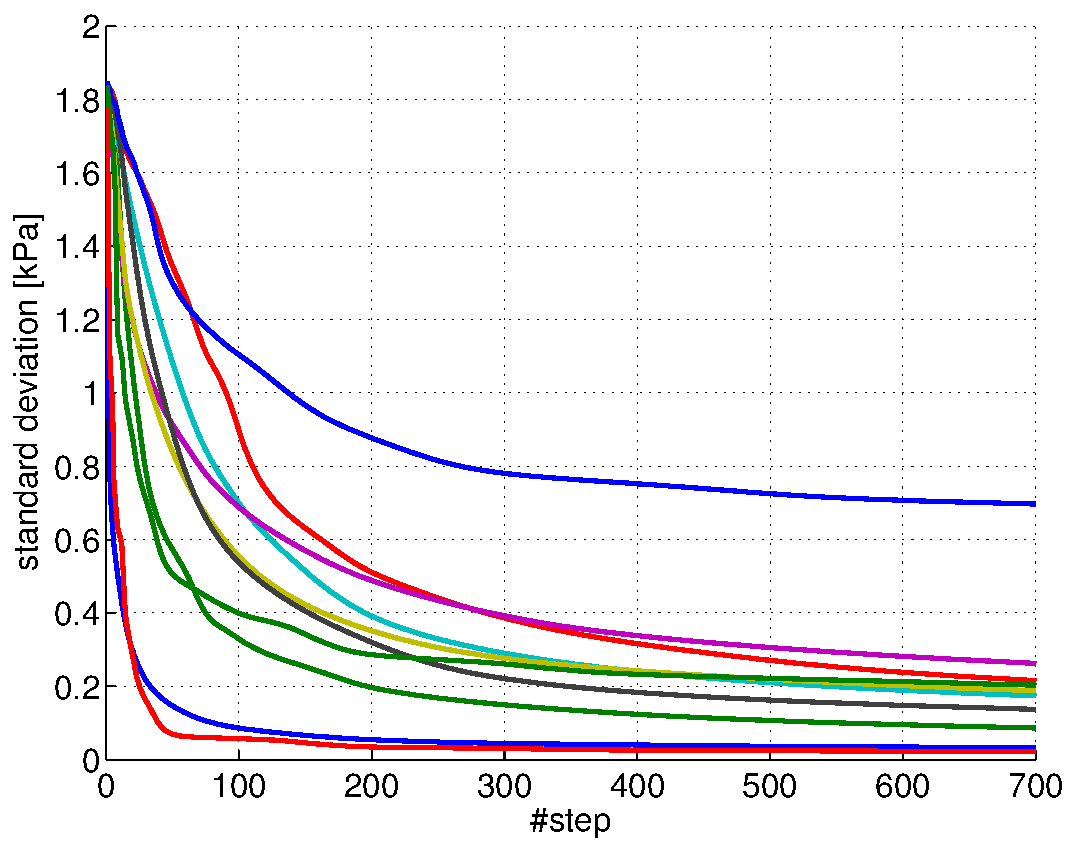
\includegraphics[width=.32\textwidth]{figs/cyl10ns_var.pdf}}
\caption{Results of the estimation of parameters for $\msb$: Ten parameters are estimated, each associated to 
one segment of the mesh. Figures (a) and (b) show the evolution of the parameter estimation as the function of the quasis-static 
incremental gravity loading without and with noise added to the observations, respectively. The dashed lines indicate the ground-truth 
and the estimation starts in the undeformed configuration. The plot (c) shows the evolution of the standard deviation 
associated to each parameter and their combinations, respectively.}%
\label{f:cyl10Estim}
\end{figure*}

\subsection{Parameter estimation}
\label{sr:estim}
The parameter estimation was performed using the ROUKF method described 
in section~\ref{sm:ROUKF} employing the implementation based on the SOFA and Verdandi frameworks. 
Two different reconstruction scenarios were tested: first, for both $\msa$ a $\msb$, the number of parameters to estimate was 
set to the number of segments, \ie\ 3 and 10 parameters each corresponding to the value of the Young's modulus of the respective segment. 
At the beginning of each estimation, the same expected value $\eexp$=\SI{6000}{\Pa} and standard deviation $\evar$=\SI{2000}{\Pa} was attributed to 
each estimated parameter. This means that the information about geometrical distribution of the heterogeneous segments was 
given as \emph{a priori} known assumption and the data assimilation was used to estimate the parameter of given pre-defined segment.

In the second scenario applied only to the mesh $\msa$, no assumption about the distribution of the heterogeneous regions was made. 
Therefore, it was necessary to consider the Young's modulus of each element as an independent parameter. Given the size of the 
mesh, 770 parameters were to be estimated by the ROUKF method.  

The correction phase of the assimilation process is directly determined by the computation of the innovation based on observations.
Given the quasi-static scenario, only positions are used as the observed quantities. 
Nevertheless, instead of using all known positions (\ie\ position of all the nodes 
in $\msa$ and $\msb$), we limited the observations to 10 points located on the axis of each cylinder as shown in Fig.~\ref{f:cylScreens}. 
Therefore, the Kalman gain computed by the ROUKF calculates the innovation using the actual Euclidean distance between the position of 10 points 
mapped to the actual deformed configuration of the cylinder estimated by the data assimilation process, and the real positions of 
the points computed from the synthetic observation data generated during the forward simulation. In order to mimic the 
real scenarios where the observations usually suffer from noise, the elements of the observation vectors were modified using 
Gaussian white noise with standard deviation $\text{Var}_\text{noise}$ = \SI{2}{\mm}.



\begin{figure*}[t!]%
\centering%
\subfigure[]{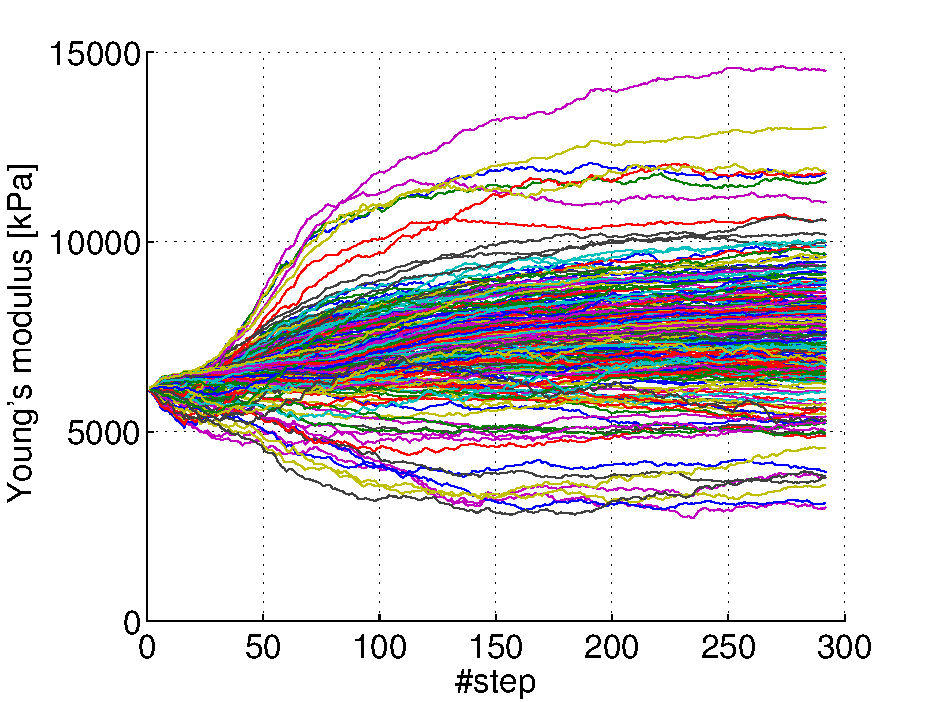
\includegraphics[width=.32\textwidth]{figs/cyl3EA_seg3.pdf}}
\hfill
\subfigure[]{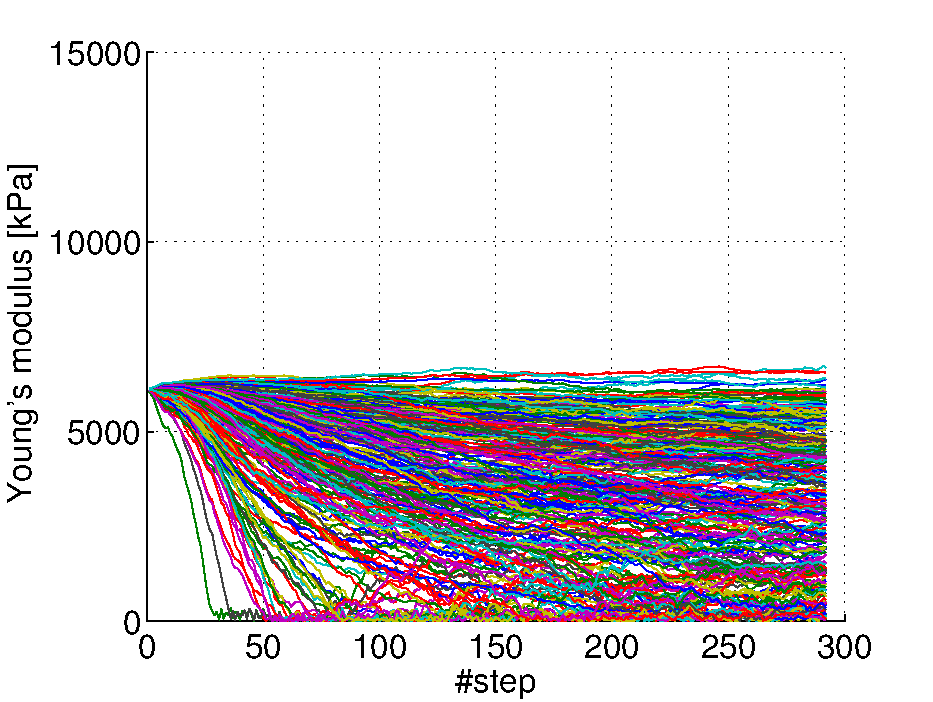
\includegraphics[width=.32\textwidth]{figs/cyl3EA_seg2.pdf}}
\hfill
\subfigure[]{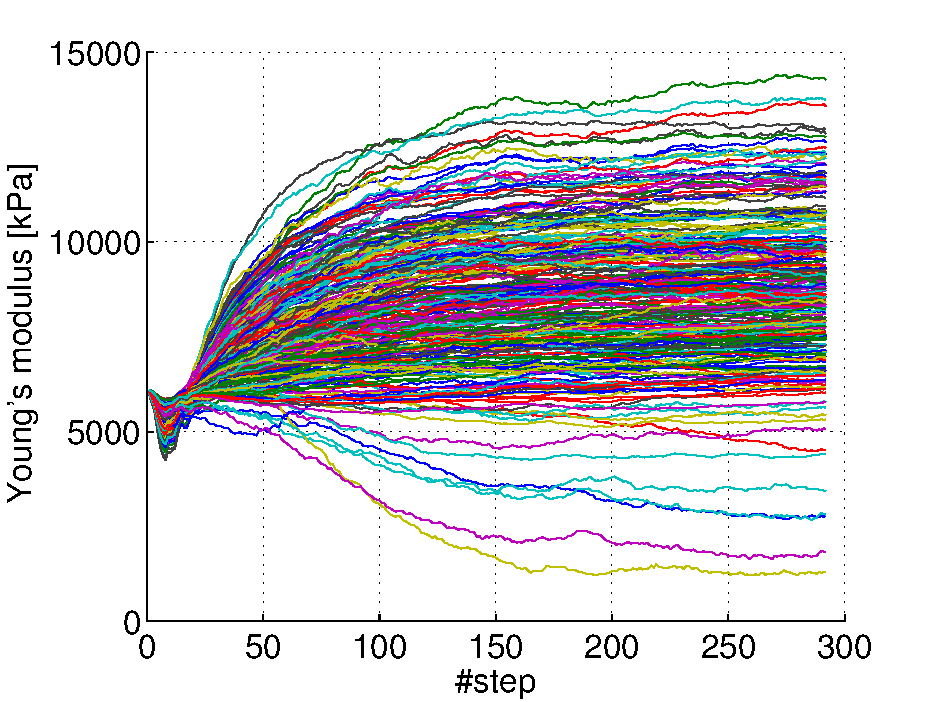
\includegraphics[width=.32\textwidth]{figs/cyl3EA_seg1.pdf}}
\caption{Evolution of the elasticity estimation independently for each element as functions of the quasi-static incremental gravity loading.
The three plots (a), (b) and (c) shows the evoluation of estimations associated to elements from segment 1, 2 and 3. We recall that 
the Young's moduli used in the forward simulations were $\{8,2,10\}$\,kPa}.%
\label{f:cyl3EAsegs}
\end{figure*}


\subsection{Estimation of Elastic Modules per Segment}
\label{sr:segment}
The results obtained for the estimation of elastic modules associated to each segment are presented in Fig.~\ref{f:cyl3Estim} for 
$\msa$ and in Fig.~\ref{f:cyl10Estim} for $\msb$. In the case of $\msa$, the estimated expectations converge to the real values 
used in the forward simulation even with added noise. This is also reflected by the fact that the standard deviation associated to each 
parameter quickly approaches zero. In the case of $\msb$, the situation is more complicated as for some parameters, the convergence is clearly 
not achieved. However, these parameters can be identified (without knowing the ground-truth) from the respective standard deviation which 
remain important event after large number of steps, thus indicating significant uncertainty associated with the estimation. 
Nevertheless, given the limited number of the observation points which is equivalent to the number of estimated parameters, 
the results signal an interesting level of robustness of the estimator. 

\subsection{Estimation of Elastic Modules per Element}
\label{sr:element}
In this evaluation, the elasticity of each element of the mesh $\msa$ was estimated as an independent parameter. Thus, 770 parameters were estimated in total. 
The expected values were stored in each step of the data assimilation process. In order to facilitate the visualization, 
the histories of parameter estimations were plotted separately for each segment as shown in Fig.~\ref{f:cyl3EAsegs}. 
It should be emphasized that the curves were regrouped \wrt\ the segments as a part of data post-processing and so no \emph{a priori} 
information about the location of given element \wrt\ the segments was given during the data assimilation process. 
In order to get more quantitative assessment, Fig.~\ref{f:cyl3EAmeans} shows the mean curves computed for each segment 
from Fig.~\ref{f:cyl3EAsegs}. The preliminary evaluation suggests that the data assimilation based on ROUKF is capable of 
reliable estimation of the elasticity parameters even for the somewhat extreme case where the elasticity of each element of the 
mesh is treated as an independent parameter to be estimated. For the sake of clarity, we are not plotting the standard deviation
of the parameters, however, we plan to perform statistical evaluation of these quantities which is beyond the scope of this paper. 

\subsection{Performance of the method and parallelization}
\label{sr:perf}
The performance of the method was evaluated using a single cluster node equipped with 16 CPUs AMD Opteron 6274 running at \SI{2.2}{\giga\hertz}.
The procedures were executed at least 3 times and mean measured value is reported. 
In order to quantify the performance of the data assimilation, we first report the performance of the 
forward simulation: in the case of $\msa$, the forward simulation in SOFA was running at \SI{50}{FPS} while the data assimilation using the 
\emph{simplex} type of the sigma points was running at about \SI{20}{FPS}. Similarly, the direct simulation using $\msb$ 
was running at \SI{20}{FPS}. In this case, the data assimilation was much slower: the refresh rate did not exceeded \SI{1}{FPS}. This 
is however expected due to larger number of parameters to be estimated.

As for the scenario where the elastic modules were estimated per elements, the running time is significantly longer: one step of the data assimilation 
took about 15 s for the simplex, and 25 s for the star type of the sigma points. 

The numbers reported above were measured for the sequential execution of the data assimilation. The impact of the parallelization 
is depicted in Fig.~\ref{f:parallel} where the estimation of 10 parameters using the mesh $\msb$ was executed using 1, 4, 8, 12 and 16 threads
for all the three types of the sigma points. Since the parallelization was performed only for the predictive case, the plot 
indicates the limits this approach, since even for the \emph{star} ROUKF, no speed-up is observed when the number of threads exceeds 12, 
despite the fact that the model step (performed in parallel) was executed 21 times. 
